\section{Static Load Balancing}
\label{sec:static-load-balancing}

% technical details
In the original ParSplice implementation, each cache node uses an unlimited
amount of memory to store segment coordinates. We limit the size of the cache
using an LRU eviction policy, where the penalty for a cache miss is retrieving
the data from the persistent database.  We evict keys (if necessary) at every
operation instead of when segments complete because the cache fills up too
quickly otherwise.

% results: cache size trade-offs
\begin{figure}[t]
  \noindent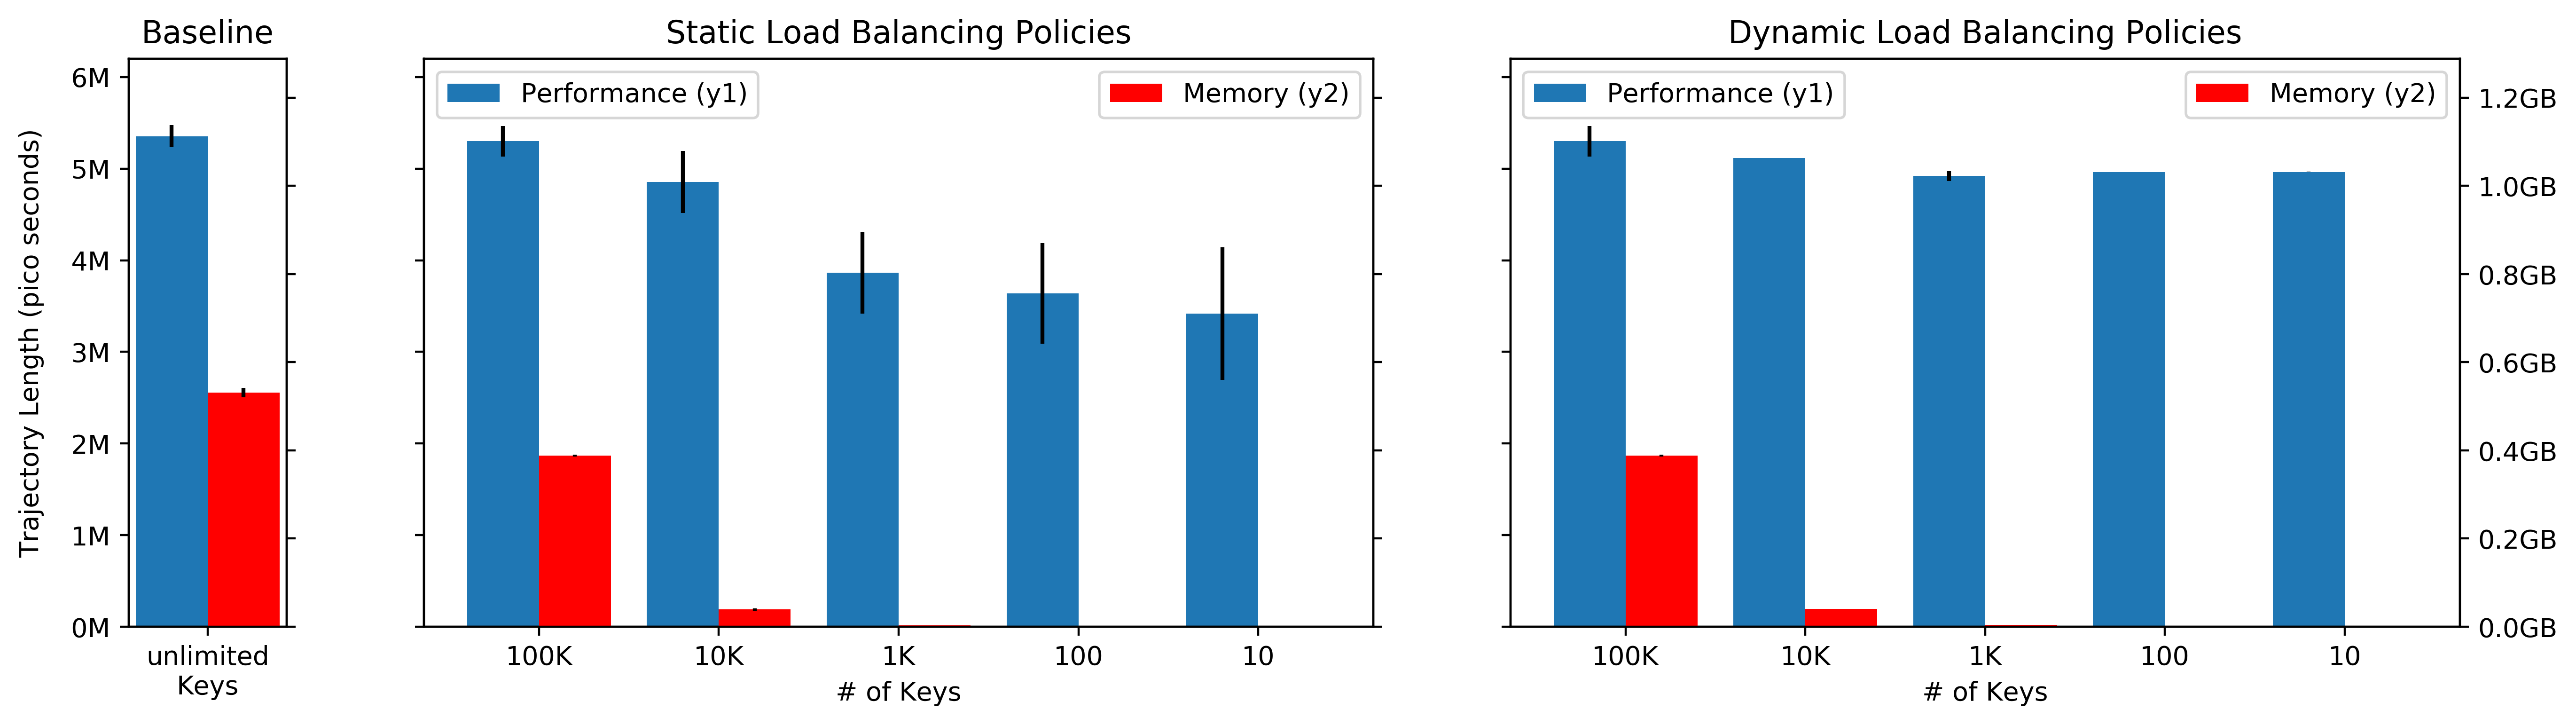
\includegraphics[width=0.5\textwidth]{figures/methodology-tradeoff.png}\\

  \caption{The performance and resource utilization trade-off for different
cache sizes. ``Baseline" is
ParSplice unmodified and the ``Policy: Constrain Cache Size" graph limits the
size of the cache to save memory.  \label{fig:methodology-tradeoff}}

\end{figure}

The results for different cache sizes for a growth rate of \(\Delta_1\) over a
2.5 hour run across 256 workers is shown in
Figure~\ref{fig:methodology-tradeoff}.  ``Baseline" is the performance of
unmodified ParSplice  measured in trajectory duration (\(y\) axis) and
utilization is measured with memory footprint of just the cache (\(y2\) axis).
The other graph shares the \(y\) axis and shows the trade-off of constraining
the cache to different sizes.  The error bars are the standard deviation of 3
runs. 

% results: raw numbers
Although the keyspace grows to 150K, a 100K key cache achieves 99\% of the
performance. Decreasing the cache degrades performance and predictability.
While this result is not unexpected, it nonetheless achieves our goal of
showing the benefits of load balancing keys across nodes and that smaller
caches on each node are an effective way to save memory without completely
sacrificing performance.
